\documentclass[11pt,journal,compsoc]{IEEEtran}

\usepackage{ctex}

\usepackage{graphicx}

\usepackage{url}

\usepackage{hyperref}

\usepackage{enumitem}

\usepackage{amssymb}

\usepackage{indentfirst}

\setlength{\parindent}{0em}

\usepackage{float}

\begin{document}


Informatics


\section{Processors \& Memories}


\subsection{Von Neumann Principle}

程序 和 数据 储存在 单一独立的储存单元 内存 中,它们通过 共同的总线 进行访问。它们在 物理上 是相同的,计算机根据 指令 来处理它们,易重新编程。


\subsection{Von Neumann Loop}

\begin{enumerate}
    \item CPU 从内存中取指令 Fetch
    \item 解码以确定操作 Decode
    \item 执行 Execute
    \item 从内存中取
    \item 写回内存
\end{enumerate}

重复,直到程序结束。CPU 在获取 指令和数据 之间交替,降低速度。


\subsection{Von Neumann Architecture}

存储器、运算器、控制器、输入设备和输出设备五部分组成计算机。运算器和控制器合称为中央处理器。


\subsection{Harvard}

此架构使用 两个不同的储存器 来 分别储存 指令和数据,不同的总线进行访问,速度更快,成本更高。


\subsection{CISC}

Complex / Reduced Instruction Set Computer

复杂指令集的每个指令可执行若干低端操作,指令数目多而复杂,周期长,更适合复杂操作,简单操作可能浪费时间。

原因:寄存器昂贵,尽可能使单个指令做更多的工作


\subsection{RISC}

精简指令集针对流水线化的处理器优化,指令数目少,周期短,更好的并行执行,编译器的效率更高,便宜节能。

x86 对简单指令有硬件加速。

ARM V7 和之前没有 AES。


\subsection{Commands}

一组指示处理器执行特定操作的二进制代码,包含 OpCode 和 Operand 两部分,汇编。


\subsection{Registers}

CPU 内部用来存放临时数据的内存,非常快,很小。x86-64架构有 16 个通用寄存器。

CPU $\leftrightarrow$ 寄存器 $\leftrightarrow$ 缓存 $\leftrightarrow$ 内存


\subsection{Pipeline}

指令流水线,将每条指令分解为多步,每个阶段可以并行执行不同的指令,从而实现几条指令并行处理。指令仍是一条条顺序执行,一个时钟周期内可以执行一条完整的指令。当一个指令在 Execute 时,另一个指令可以开始执行 Decode,以此类推。


\subsection{Superscalar}

在单个核心中有多个流水线,一个时钟周期内执行多个指令,并行地对多条指令进行流水处理。


\subsection{Memories}


\subsubsection{}{按物理结构}

\begin{description}
    \item[SRAM] Field-Effect Transistor、无需刷新、极快、\\ 昂贵、CPU 缓存

    \item[DRAM] Capacitance、周期刷新、内存

    \item[ROM] 只读

    \item[Programmable ROM] 内部有熔丝,利用电流将其烧断,以写入数据,一经烧断便无法恢复

    \item[Erasable PROM] 利用高电压将数据写入,有透明窗口,曝光于紫外线时抹除数据

    \item[OneTime PROM] 与 EPROM 一样,但无透明窗

    \item[Electrically EPROM] 使用高电场来抹除

    \item[Flash] NAND($!\&$ SSD)与 NOR($!\|$ BIOS)型、\\ 寿命有限、较慢
\end{description}


\subsubsection{按组织方式}

\begin{description}
    \item[Serial] 比如 Magnetic Tape、密度高、速度慢、\\ 不能随机存取

    \item[Parallel] 比如 Disk、同时读写多个比特

    \item[Distributed] 信息存储于多个独立且互不干扰的 \\ 设备中、可靠性、扩展性

    \item[Hierarchical] 高效率,比如 Cache -> RAM -> ROM
\end{description}


\subsubsection{按访问类型}

\begin{description}
    \item[Direct Memory Access] 不经过 CPU,比如显卡的 DirectStorage

    \item[Sequential Access Memory] 磁带

    \item[Random Access Memory] 内存
\end{description}


\section{Peripherals \& Storage \& I/O}


\subsection{Storage}

\subsubsection{By Construction}

\begin{description}
    \item[Solid] SSD, Flash 速度快

    \item[Optical] CD, use Laser

    \item[Magnetic] HDD, Tape, Floppy 容量大
\end{description}

\subsubsection{By Operation Principle}

\begin{description}
    \item[RAM] Volatile
    \item[ROM] Non-Volatile
    \item[Sequential]
\end{description}


\subsection{Peripherals}

\subsubsection{By Functionality}

\begin{description}
    \item[Input] Keyboard, Mouse
    
    \item[Output] Monitor, Speaker

    \item[Storage] Flash Drive

    \item[Network] Router, Switch
\end{description}

\subsubsection{By Means}

\begin{description}
    \item[Wired]
    \item[Wireless]
\end{description}

还有 Bidirectional 双向设备


\subsection{Bus}

is physical pathways used by CPU and other devices to communicate.


\subsubsection{Data}

CPU \leftrightarrow RAM

CPU \leftrightarrow I/O Devices

传输数据,宽度决定一次传输多少比特,8 - 64 bits 常见


\subsubsection{Address}

沟通物理地址,宽度决定寻址的内存大小


\subsubsection{Control}

控制 CPU 和设备的:读写、时钟、中断、复位 等信号


\subsection{I/O}

handling is the process of managing the communication between CPU and devices.


\subsubsection{Programmed}

最简单,基本,低效率。CPU 直接控制 I/O 设备和 存储器 之间的数据传输


\subsubsection{IRQ}

Interrupt-Request。I/O 需要运算时,向 CPU 发送中断请求,并处理需求


\subsubsection{Direct Memory Access}


\subsection{Protocols}

传输数据的方法


\subsubsection{Parallel}

所有信号线在同一时刻传输数据 导致信号互相干扰(串扰)。传输速率提高,时钟同步和时序控制变难。

\begin{description}
    \item[Centronics] Enhanced Parallel Port 打印机通信,8 位数据总线和几个控制信号,25 PIN

    \item[Peripheral Component Interconnect] 连接外围设备,32 位 133 MB/s
\end{description}


\subsubsection{Serial}

一次传输一比特,数据沿单一信道传输,差分信号降低干扰和提高质量,增加 Lane 数量提升速率。

差分:一正一负两根线,通过电压差获取数据。

\begin{description}
    \item[Recommended Standard 232] 一条数据线发送接收,控制线用于握手和流量控制,工业

    \item[High-Definition Multimedia Interface] DP

    \item[PCI Express] x32 表示 Lane 数,32 GT/s 每 Lane
\end{description}


\subsubsection{Universal Serial Bus}

同时供电通信,即插即用,40 Gbps,Thunderbolt 兼容

\begin{description}
    \item[主从通信] Host 管理控制数据传输

    \item[层次结构] ~
    
        \begin{itemize}
            \item 物理:接口形状,功率等
            \item 链路:建立和维护通信
            \item 协议:格式等
            \item 传输:打包数据
            \item 会话:管理
            \item 应用:处理驱动程序的请求
        \end{itemize}

    \item[数据包] 传输的基本单位,Token、Data 和 Handshake

    \item[传输模式] ~

        \begin{itemize}
            \item Control:设备配置,状态查询,命令执行

            \item Bulk:大量数据,高速,延迟高

            \item Interrupt:低延迟,少量数据,实时,慢,鼠标

            \item Isochronous:音视频,固定速率和延迟,会丢包
        \end{itemize}

    \item[初始化] 识别设备,查询信息,分配地址,选择配置
\end{description}


\section{Operating Systems}

管理软硬件的软件,为程序提供基本服务,用户与硬件的中介。


\subsection{Classification}

\begin{description}
    \item[Batch] 自动化执行一系列工作(早期大型计算机)

    \item[Time-Sharing] 多用户共享资源,Time-Slicing,为每个用户分配时间片段,并发使用

    \item[Real-Time] 对事件立即作出反应,错过最后期限时:Hard Failure;Soft Tolerable

    \item[Distributed] 超算集群,多合一

    \item[Embedded] 物联网
\end{description}


\subsection{Functionality}

\begin{description}
    \item[Process] 管理进程,分配 CPU 时间,优先级

    \item[Memory] 管理虚拟内存,分配内存,内存边界

    \item[File System] 管理空间分配,控制访问,维护完整性

    \item[Device] 管理连接设备,提供标准化接口

    \item[UI] 用户互动,CLI / GUI

    \item[Security] 认证授权

    \item[Networking] 进程间,网络上通信

    \item[Error Handling] 处理错误,保持稳定
\end{description}


\subsection{Process \& Scheduling}

确保资源有效利用,为用户提供灵敏高效的环境


\subsubsection{Process Management}

创建,执行,终止

\begin{description}
    \item[Process] 一个正在执行的程序,由代码、数据和一组资源组成

    \item[Control Block] 包含进程信息,如ID,状态,优先级,内存用量等

    \item[States] 如 ready / running / waiting / terminated

    \item[Scheduler] 根据策略 从就绪队列中 决定哪个进程 应该在指定时间执行
\end{description}


\subsubsection{Scheduling Methods}

\begin{description}
    \item[First-Come, First-Served] 先到先得,对于交互式不佳,可能有长期运行的进程

    \item[Shortest Job Next] 最小化平均等待时间,有可能导致长进程长等待

    \item[Round Robin] 每个进程都有固定的 Quantum 来执行,用完后会被移到队列后方,平衡了公平和效率,适合交互

    \item[Priority Scheduling] 先执行高优先级,确保响应性

    \item[Multilevel Queue Scheduling] 每个优先级都有独立的队列,与其他方法配合

    \item[Multilevel Feedback Queue] 类似上面,但可以根据进程行为,在不同优先级队列中移动进程,比如 I/O 绑定,动态调整提高效率和响应
\end{description}


\subsubsection{Scheduling in Interactive}

优先考虑前台任务,响应性

\begin{description}
    \item[Preemptive Scheduling] 抢占式,可中断运行中的进程,把时间分配给更高优先级,及时响应输入

    \item[Dynamic Priority Adjustment] 根据行为和资源动态调整优先级,如 CPU 爆发式的 I/O 绑定可更优先

    \item[Load Balancing] 在多个 CPU 核心中分配进程,\\ 确保没有过载

    \item[Resource Reservation] 为关键进程保留 CPU 时间

    \item[Adaptive Scheduling] 动态调整使用的策略
\end{description}


\subsubsection{Aim \& Requirements}

\begin{description}
    \item[Fairness] 维持稳定平等,防止垄断

    \item[Efficiency] 最小化开销,最大化吞吐,减少上下文切换,避免 CPU 饥饿

    \item[Responsiveness] 迅速响应高优先级事件

    \item[Predictability] 确保进程在合理的时间内根据优先级和资源需求被执行,实时系统

    \item[Adaptability] 适应不断变化的系统环境,如变化的负载或新进程加入
\end{description}


\subsection{Memory}


\subsubsection{Management}

有效分配,跟踪,管理内存块,使多个进程共享内存并同时执行,确保每个进程有必要的运行资源,防止碎片,进程隔离

\begin{description}
    \item[De / Allocation] 需时分配,用完回收,防止泄漏

    \item[Organization] 将内存分为多个部分,分离不同类型的内存,如 code、data、stack,高效
\end{description}


\subsubsection{Relocation}

调整代码和数据所处的内存地址,允许它在不同的位置执行,多个进程有效分享有限的内存

\begin{description}
    \item[Static] 地址在编译或链接时被调整,产物包含最终的地址,程序只能在特定的地址被加载。简单快速但不灵活,一旦加载就不能移动

    \item[Dynamic] 运行时调整地址。加载到内存时会计算实际位置与参考位置的差异,称之为 Relocation Constant 或 Base Address,被添加到程序中每个内存的引用中。允许多个程序共享同一内存空间而不冲突
\end{description}


\subsubsection{Protection}

防止程序没有授权的情况下访问修改另一个程序的内存,确保系统稳定性,安全性和完整性。它维持进程隔离,保护敏感数据,防止非法操作导致的系统崩溃。

\begin{description}
    \item[Memory Management Unit] 硬件,将虚拟地址到物理地址。检查进程访问权限,实时内存保护。若有非法访问,则会抛出异常,让操作系统采取行动,如终止进程

    \item[Memory Protection Unit] 硬件,特别是在没有 MMU 或者简单系统中。它定义了具有特定内存访问权限的区域,并检查进程是否有权限

    \item[Virtual Memory] 每个进程都有自己的私有地址空间,与物理层分离,提供额外保护,进程无法直接访问其他内存。OS 管理虚拟内存与物理地址的映射

    \item[Access Control] OS 实现各种访问控制规则,如权限组,以限制进程访问区域

    \item[Address Space Layout Randomization] ~
    
    随机化代码与数据在内存中的位置,使攻击者更难预测布局并执行 Buffer Overflows 等攻击
\end{description}


\subsubsection{Swapping}

在 RAM 与 硬盘 之间移动数据以释放 RAM 空间的操作,是虚拟内存管理的关键部分。当 RAM 可用不足时,OS 可能会将一些不常用的数据 swapping out 或 paging out,当再次需要时,会被 in 到 RAM。

Swap 是使用磁盘空间来扩展 RAM 的有效方法,然而会减慢系统速度,所以 OS 使用复杂的算法,根据频率,内存用量等因素决定哪些部分可以且何时进行交换。同时结合硬件,如 Translation Lookaside Buffers 和 MMU 来优化性能。

TLB:CPU 的一种缓存,由 MMU 用于改进虚拟到物理地址的转译速度


\subsubsection{Paging}

将虚拟内存划分为固定大小的块,Pages。物理内存也被划分,Frames。它们具有相同大小,通常是 2 的幂。OS 维护 Page Tables,将 Pages 映射到 Frames,供 MMU 查询。

优点:

\begin{description}
    \item[Efficient Allocation] 通过分块,避免外部碎片,简化操作

    \item[Virtual Memory] 实现的基础

    \item[Protection] 每个进程都有自己的 Page Table,OS 可以为每个 Page 设置权限

    \item[Demand Paging] 只有在实际使用时才加载 Page
\end{description}

开销:

\begin{description}
    \item[Management] Page Tables 需要额外内存和处理

    \item[Translation] 映射开销

    \item[Page Faults] 当引用不在物理内存的 Page 会引发,需要 OS 从磁盘加载,比较缓慢
\end{description}


\section{Network Architectures}


\subsection{Layers}


\subsubsection{Open Systems Interconnection}

\begin{enumerate}
    \item Physical

    电信号,电压,介质规范
    
    \item Data Link

    纠错,流量控制,包含 LLC 和 MAC 两个子层

    \item Network

    不同网络之间的路由和转发,寻址,拥堵控制,数据包排序,IP 在此层

    \item Transport

    可靠端到端传输,错误检查,流量控制,数据分段,TCP 和 UDP

    \item Session

    管理 App 之间的连接,处理中断恢复

    \item Presentation

    处理数据加密,压缩,转换为 App 可理解的格式

    \item Application

    提供接口,高级协议,如 HTTP
\end{enumerate}


\subsubsection{Logical Link Control}

在 一层 和 MAC 层之间提供接口

\begin{description}
    \item[Multiplexing] 增加一个协议标识符,使多个上层协议共享同一个 MAC

    \item[Error Control] MAC 主要处理错误,但 LLC 也可以重传

    \item[Flow Control] 控制速率,防止缓冲区溢出
\end{description}


\subsubsection{Media Access Control}

管理数据如何在介质上传输

\begin{description}
    \item[Addressing] 为设备中每一个接口分配一个唯一的硬件地址,48位,用于识别和引导数据流

    \item[Framing] 将来自上层的内容封装,header(控制,MAC地址)、payload、trailer(校验)

    \item[Error Detection] 使用不同算法检测损坏 Frame,丢弃和重传

    \item[Access Control] 避免冲突,有效利用带宽
\end{description}


\subsubsection{TCP/IP}

TCP/IP 协议是一个协议簇,包含很多协议,UDP TCP ICMP IP...

\begin{enumerate}
    \item Link (1, 2)
    \item Internet (3)
    \item Transport (4)
    \item Application (5, 6, 7)
\end{enumerate}


\subsection{Hardware}

\begin{description}
    \item[Network Interfaces] 1,网卡,通过网络介质传输数据,分配 MAC 地址

    \item[Repeaters] 1,中继,放大信号,扩大覆盖范围

    \item[Bridges] 2,桥接,连接两个独立的网段。根据 MAC 地址,创建过滤表以减少不必要的流量,\\ 并转发数据

    \item[Hubs] 1,集线,连接网络中多个设备,并将数据转发给所有连接的设备,没有过滤等功能

    \item[Switches] 2,交换,连接网络中多个设备,根据 MAC 地址转发和过滤,比 Hub 高效

    \item[Routers] 3,路由,连接多个网络并根据 IP 转发,使用路由算法确定最佳路径,提供 NAT,防火墙,QoS等功能
\end{description}


\subsection{Ethernet}

它是有线 Local Area Network (LAN) 技术,局域网通信标准,1 / 2 层。

\begin{description}
    \item[Topology] 星形结构,设备连接到中央设备,如交换机

    \item[Media] 支持各种介质,Coaxial、Twisted-pair、Fiber-Optic,RJ-45 接口

    \item[Speed] 100 M / 1 G / 10 G 等

    \item[Frame] Preamble, Destination / Source MAC address, EtherType (indicating the payload's protocol), Payload (data), Frame Check Sequence.

    \item[MAC] Carrier Sense Multiple Access with Collision Detection,在传输之前会监听空闲的通道,如果发生多个设备同时传输,则在重试之前会等待一段随机时间
\end{description}


\subsection{802.11 / WiFi}

\begin{description}
    \item[a] 5 GHz,54 Mbps,不易受干扰,范围小

    \item[b] 2.4 GHz,11 Mbps,易干扰,范围广

    \item[g] 2.4 GHz,54 Mbps

    \item[n] 2.4 and 5 GHz,600 Mbps,四个 Spatial 流,MIMO

    \item[ac] 5 GHz,6.93 Gbps,八个流,Multi-User MIMO,同时向多个设备传输,160 MHz 信道,256-QAM

    \item[ax] 2.4 and 5 GHz,9.6 Gbps,OFDMA,BSS Color
\end{description}


\subsubsection{Multiple Input Multiple Output}

发射端的多个天线各自独立发送信号,同时在接收端用多个天线接收并恢复原信息,多根天线增加吞吐量和范围


\subsubsection{Quadrature Amplitude Modulation}

在两个 Orthogonal 载波上进行幅度调制的调制方式,通常是相位差为 90 度的正弦波,星座图上每一个星座点对应发射信号集中的一个信号,星座点数越多,能传输的信息量就越大


\subsubsection{Orthogonal Frequency Division Multiple Access}

将高速的数据流分成多个低速数据流,在多个正交子载波上并行传输


\subsubsection{Basic Service Set Coloring}

标签,用于区分来自不同网络的信号。在高密度环境中,不同 AP 的信号会相互干扰,降低性能。通过为每个 BSS 分配一个颜色标识,减少相邻无线网络之间的干扰


\subsection{Internet Protocol}

不可靠的无连接协议网络协议,不保证交付,不在发送数据前建立连接。第三层,寻址、路由、打包


\subsubsection{IPv4}

Header 最小 20 bytes:

\begin{description}
    \item[Version] 4 bit

    \item[Internet Header Length] 4

    \item[Type of Service] 8

    \item[Total Length] 16

    \item[Identification] 16,Important for Fragmentation and Reassembly

    \item[Flags] 3,—,[1] 保留,[2] 不要分段,[3] 后面还有

    \item[Fragment Offset] 13,—,片段的索引

    \item[Time to Live] 8,在丢弃前最大跳数

    \item[Protocol] 8,TCP 6,UDP 17

    \item[Header Checksum] 16,每一跳都重新计算和校验

    \item[Source IP] 32

    \item[Destination IP] 32

    \item[Options / Padding] var
\end{description}


\subsubsection{IPv6}

IPsec,更好的 QoS,Stateless IP 配置,Multicast and Anycast

定长 Header 40 byte:

\begin{description}
    \item[Version] 4,6

    \item[Traffic Class] 8,QoS

    \item[Flow Label] 20,标记具有相同 QoS 的序列

    \item[Payload Length] 16

    \item[Next Header] 8,如 TCP 头

    \item[Hop Limit] 8,TTL

    \item[Source IP] 128

    \item[Destination IP] 128
\end{description}


\subsection{Network Address Translation}

Types of NAT:

\begin{description}
    \item[Static] 一对一固定公网

    \item[Dynamic] 一对一动态公网

    \item[Port Address Translation] 常用,共享公网
\end{description}

NAT Behavior:

\begin{description}
    \item[Full Cone] 任何外部都可以与映射端口的内部通信

    \item[Restricted Cone] 内部先向外才能通信

    \item[Port Restricted Cone] 相同端口号

    \item[Symmetric] 每一个连接都分配不同的 IP 和 端口
\end{description}


\subsection{Classless Inter-Domain Routing}

无类型域间选路,Classful 是 A (x.0.0.1) B (x.x.0.1) C (x.x.x.1)

子网掩码用于区分网络和主机部分,255.255.255.0 的二进制表示为 11111111.11111111.11111111.00000000,24 个 1 是网络;8 个 0 是主机,则掩码的前缀长度为 24。所以 192.168.1.1 和 255.255.255.0 的 CIDR 为 192.168.1.1/24

127.0.0.0/8 是一个网段,子网掩码为 255.0.0.0。这个网段包含了 127.0.0.0 到 127.255.255.255 的所有 IP 地址。

127.0.0.1/32 是一个单独的 IP 地址,子网掩码为 255.255.255.255,表示只有一个 IP 地址 127.0.0.1。127.0.0.1 也被称为本地回环地址(loopback address)


\subsection{Routing}

路由,在网络中选择路径来发送网络流量的过程,确保数据包能有效和准确地从源头传递到目的地

路由表,存储通往不同网络目的地路径信息的数据结构,当路由器收到数据包时,它在其路由表中查找目的地IP地址,以确定转发数据包的下一跳,它包含:

\begin{description}
    \item[Destination / Mask] 目的地网络,可以是一个地址也可以是网段

    \item[Protocol] 获取到本条路由信息的方式,Direct(0),Static(60),OSPF(10)等

    \item[Preference] 对于不同的 路由协议 进行区分,越低越可靠

    \item[Cost] 某个路由都是从相同的协议收到时,则比较开销,不同协议不可比,越小越优

    \item[Next Hop] 下一个节点

    \item[Interface] 出口设备
\end{description}


\subsubsection{Open Shortest Path First}

在 OSPF 前,广泛使用 RIP(Routing Information Protocol)作为内部网关协议。由于 RIP 是基于距离矢量算法的路由协议,存在着收敛慢、路由环路、可扩展性差等问题,所以被 OSPF 取代。作为基于链路状态的协议,优点:

\begin{enumerate}
    \item 组播形式收发报文,减少对其它不运行 OSPF 路由器的影响
    \item CIDR
    \item 对等价路由进行负载分担
    \item 报文加密
\end{enumerate}


\subsubsection{Border Gateway Protocol}

在 Autonomous System 间交换 Network Layer Reachability Information 的协议。当运行于同一 AS 内部时,被称为 Internel BGP,不同 AS 之间时,称为 Externel BGP。

发送 BGP 报文的路由设备称为 Speaker,它接收或产生新的路由,并 Advertise 给其他邻居。BGP 通过 TCP 传递,有Open、Update、Notification (Stop)、Keepalive 和 Route-refresh五种报文类型


\subsection{Transmission Control Protocol}

Header 20 byte:

\begin{description}
    \item[Source / Des Port] TCP 不记录 IP

    \item[Sequence Num] 解决 Reordering,已传输的字节数会增加它

    \item[Acknowledgement Num] 确认收到

    \item[Flags] 包的类型,操控状态机

    \item[Window] 滑动窗口,流控
\end{description}


\subsubsection{Handshake}

网络上的传输是没有连接的,只有 连接状态。

\begin{description}
    \item[三次握手] SYN - SYN - ACK,同步 Inital Seq Num,用这个序号来拼接数据。

    当服务器在 SYN-RCVD 状态但没有收到最后的 ACK 时,会以翻倍的时间重试。Flood 攻击则是创建大量 SYN 连接并下线,可以把 SYN 队列占满。但可以通过 tcp-syncookies 临时应对:通过 Src Des 和 时间戳 制作一个特殊的 Seq Num 发回去,正常连接会把 SYN Cookie 返回,并直接建立连接

    \item[四次挥手] 其实是两次 FIN - ACK,只不过有一方是被动的。
    
    如果双方同时 FIN,则进入 Closing 状态,等待 Maximum Segment Lifetime (30s) * 2,确保对方收到了 ACK,有足够的时间让此连接不会跟后面的新连接混淆(有些路由会缓存 IP 数据包,如果连接被重用,那么延迟收到的包就可能与新连接混淆)
\end{description}


\subsubsection{重传}

Receiver 发送给 Sender 的 ACK 只能确认最大的连续收到的包,比如发送了 1 2 3 4 5,收到了 1 2,则回复 ACK 3(是期望接收的下一份数据),随后又收到了 4,但是没有收到 3,此时:

\paragraph{Timeout} ~

当 Sender 超时没收到 ACK 3,则

\begin{itemize}
    \item 重传 3
    \item 重传 3 4 5
\end{itemize}

两种方案,但是都要等超时,有可能会很久

\paragraph{Fast Retransmit} ~

所以,不以时间驱动,如果发送方连续收到三次相同的 ACK,就重传

收到 1,回 ACK 2;收到 3,回 ACK 2;4 5 收到,回 ACK 2。则重传 2,回 ACK 6

只解决了时间问题,但是不知道重传一个还是剩下全部

\paragraph{Selective ACK} ~

所以在 TCP 头里面加一个 SACK,汇报已收到的数据,是一个范围。但是 Receiver 有权 Reneging 数据,所以 Sender 也不能完全依赖 SACK,且 SACK 会消耗 Sender 的资源

\paragraph{Duplicate SACK} ~

使用 SACK 告诉 Sender 有哪些数据被重复接收了,让其知道

\begin{enumerate}
    \item 是发出去的包丢了,还是回来的ACK包丢了

    \item Timeout 是否太小了

    \item 网络上出现了 先发的包后到 Reordering 的情况

    \item 网络上是不是把数据包给复制了
\end{enumerate}


\subsubsection{Advertised-Window}

这个字段是 Receiver 告诉 Sender,自己还有多少缓冲区可以接收数据。于是 Sender 就可以根据这个 Receiver 的处理能力来发送数据,而不会导致 Receiver 处理不过来。

如果变成 0 了,则 Sender 会每隔一段时间发送 Zero Window Probe 给 Receiver 来探测对方最新 Window 大小,到一定次数以后会断开连接

Silly Window Syndrome,如果得到的窗口太小了,那么就会当作没有,等到 Window Size >= MSS。如果网络包可以塞满 Maximum Transmission Unit 则可以用满整个带宽,而除去 TCP/IP 头,就得到 Max Segment Size。对于一些需要小包场景的程序,SSH,会关闭 Nagle


\subsubsection{Congestion Handling}

TCP不是一个自私的协议,当拥塞发生的时候,要做自我牺牲

\paragraph{Slow Start} ~

刚加入网络的连接,缓慢地提速

\begin{enumerate}
    \item Congestion Window = 1,表明可以传一个 MSS 大小的数据

    \item 每当收到一个 ACK,cwnd++

    \item 每当过了一个 Round Trip Time,cwnd * 2

    \item Slow Start Threshold 是一个上限,当 cwnd >= ssthresh 时,就会进入 拥塞避免算法
\end{enumerate}

\paragraph{Congestion Avoidance} ~

一般 ssthresh 的值是 65535 kb,当cwnd达到这个值时后

\begin{enumerate}
    \item 收到一个ACK时,cwnd + 1 / cwnd

    \item 当每过一个RTT时,cwnd++
\end{enumerate}

\paragraph{当拥塞时} ~

超过 Retransmission TimeOut 则

\begin{itemize}
    \item sshthresh = cwnd / 2
    \item cwnd = 1
    \item 进入慢启动
\end{itemize}


\subsection{User Datagram Protocol}

Header 8 byte:

\begin{description}
    \item[Src Port] 在需要对方回信时

    \item[Des Port] 

    \item[Length] 

    \item[Check Sum] 
\end{description}

特点:

\begin{description}
    \item[无连接] 不维护连接状态

    \item[没有拥塞控制] 可容忍数据丢失,但不能有较大延迟的实时应用

    \item[不可靠] 没有确认 / 重传机制

    \item[面向 Datagram] 应用层来的报文,添加 Header 后直接传递到 IP 层,反之亦然,既不合并也不拆分,不可分割
\end{description}

校验:

UDP 校验和 的计算方法与 IP 的计算方法,都是 二进制反码运算求和 再取反。但不同的是,IP 校验和只检验 IP 数据报 和首部,但 UDP 的校验和是把 伪首部 和 数据 一起校验

有一个伪首部包含

\begin{description}
    \item[Src IP]

    \item[Des IP] 

    \item[0] 

    \item[协议号] 17

    \item[数据报长度] 
\end{description}


\subsection{Quality of Service}

在有限的带宽资源下,QoS 针对网络中有突发流量时需要保障重要业务

业务可以分为:

\begin{description}
    \item[实时] 通常占据固定带宽,对稳定性要求较高

    \item[非实时] 行为难预测,经常出现突发流量,导致网络质量下降,引起拥塞,增加延迟,丢包率
\end{description}

度量指标:带宽,时延,抖动,丢包率


\subsubsection{服务模型}

QoS 模型不是一个具体功能,而是端到端 QoS 设计的一个方案。只有当网络中所有设备都遵循统一的 QoS 服务模型时,才能实现端到端的质量保证。

\begin{description}
    \item[Best-Effort] 最简单模型,用户可以在任何时候,发出任意数量的报文,网络尽力传递,不提供任何保证,适用于要求不高的业务,默认

    \item[IntServ] 在用户发送报文前,需要通过 Signaling 向网络申请特定的 QoS 服务,网络根据请求预留资源。在收到确认信息后,用户才开始发送报文

    其使用了 Resource Reservation Protocol 在整条线路上预留资源,只有所有的网元都确认,路径才能建立

    \item[DiffServ] 将流量分类,享受不同的处理,同一类业务会被聚合起来统一发送,常用

    业务流的分类和汇聚工作在网络边缘节点完成,其通过多种条件,如源 / 目的地址,协议类型等,灵活的对报文进行标记,而其他节点只需要识别报文中的标记,即可进行资源分配和流量控制
\end{description}


\subsection{Domain Name System}


\subsubsection{层级结构}

匿名根 -> 顶级域名 (通用 / 国家)-> 子域

最开始的域名最后都是带了点号的,比如 www.kernel.org. ,表示根域名服务器


\subsubsection{域名服务器}

\begin{description}
    \item[根] 全球共有 13 个不同 IP 地址的最高层次的域名服务器,从 a 一直到 m,ICANN,Anycast

    根 NS 知道所有的 顶级 NS 的地址。向 Root 请求解析 aloen.to,则会返回 .to 的 Top NS,再向其请求 aloen 的 DNS 记录

    \item[顶级] 负责该顶级域名下注册的二级域名解析

    \item[Authoritative] 子域名解析

    \item[本地] 主机发出 DNS 查询时,首先发给本地 NS
\end{description}

查询 DNS 但服务器没有结果:

\begin{description}
    \item[Iterative] DNS 服务器询问其他服务器
    \item[Recursive] 返回另一个 DNS 服务器地址
\end{description}


\subsubsection{为什么用 UDP}

节省网络资源,一个请求一个应答。DNS 数据包较小,不需要分包,只需要考虑丢包和重试。DNS 报文允许填入序号,请求和其应答报文的序号相同。


\subsubsection{常见记录类型}

\begin{description}
    \item[Address] 映射到 IPv4

    \item[AAAA] IPv6

    \item[Canonical NAME] 映射到另一个域名,别名

    \item[Mail Exchange] 射到邮件服务器

    \item[NS] 指定该域名的授权域名服务器

    \item[TXT] 存储关于域名的任意文本信息

    \item[Pointer] IP 反查
\end{description}


\section{Network \& Security}


\subsection{Data Security}

数据 Integrity,Confidentiality 和 Availability

\begin{description}
    \item[Encryption]
    \item[Access Control]
    \item[Backup]
    \item[Data Loss Prevention Tool] 检测和防止敏感数据的非法转移和泄露
    \item[Data Masking] 使用虚构的数据替换敏感信息
\end{description}


\subsection{Service Security}

免受如 APP,API 的未经授权访问或破坏与漏洞

\begin{enumerate}
    \item 定期进行漏洞扫描和补丁

    \item 在软件开发时进行安全测试

    \item 部署防火墙,IDS,IPS

    \item 网段隔离

    \item 对设备和程序进行安全配置
\end{enumerate}


\subsection{Physical Security}

防止盗窃,损坏,未经授权的访问

\begin{description}
    \item[安全设施] 访问控制,监控摄像,报警器

    \item[访问控制系统] 读卡器,生物识别等

    \item[安保人员] 监视和 Patrol

    \item[环境控制] Fire Suppression Systems,Uninterruptible Power Supplies,Air Conditioning

    \item[Asset Management \& Tracking]
\end{description}


\subsection{Security Risks of the Internet}

\begin{description}
    \item[Data Breaches] 未经授权的访问,导致身份信息被盗,财产损失等

    \item[Malware] Viruses, Worms, Trojans, Ransomware, Spyware

    \item[Social Engineering]

    \item[Distributed Denial of Service] 流量攻击

    \item[Insider Threats] 员工权限滥用
\end{description}


\subsection{Classic Encryptions}

\begin{description}
    \item[Caesar Cipher] 偏移替换,每个字母都有固定替换

    \item[Vigenère] 由一些偏移量不同的凯撒密码组成
\end{description}


\subsection{Symmetric Cryptography}


\subsubsection{Advanced Encryption Standard}

密钥长度可以是 128 192 256 位,加密过程简单描述:

\begin{description}
    \item[SubBytes] 将明文中每个字节替换成一个固定的,从 S盒 中查到的值
    
    \item[ShiftRows] 将每行的字节循环位移,使得每个字节都出现在不同的列

    \item[MixColumns] 将每列中的字节进行线性变换,使得每个字节都参与到混淆中

    \item[AddRoundKey] 将每一轮的密钥与每个字节进行异或操作,以增加强度
\end{description}

128 位的密钥 10 轮加密,192 位 12 轮,256 位 14 轮

在逆变换中,只有 AddRoundKey 与加密过程相同


\subsubsection{Substitution Box}

代换盒,由一张固定的表格构成,用于将输入的位序列映射到输出的位序列。在 AES 中,S 盒是通过多种加密学原理和技术精心构造的,以确保其具有良好的加密性质和统计性质。其包含了 256 个元素,每个元素都是一个 8 位的二进制数


\subsection{RSA}

三个人名

组成:

\begin{description}
    \item[Message] $M$

    \item[Ciphertext] 密文 $C$

    \item[Public / Private] Key

    \item[Encryption / Decryption] 算法
\end{description}

产生密钥:

\begin{enumerate}
    \item 随机选择两个不同的素数,$p = 103$,$q = 97$

    \item $n = p * q = 9991$

    \item 计算欧拉函数 $\varphi(n) = (p - 1)(q - 1) = 9792$

    \item 随机选择一个 $e = 1213$,$\varphi(n)$ 与 $e$ coprime ($gcd(a, b) = 1$) 且 $1 < e < \varphi(n)$

    \item 求 $ed - k\varphi(n) = 1$ 整数解:$k = 510, d = 4117$

    \item 公钥 (e, n) = (1213, 9991)
    
    \item 私钥 (d, n) = (4117, 9991)
\end{enumerate}

加密:

令 $M = 6$,得到 $C = M^e (mod ~n)$

$= 6^{1213} (mod ~9991) = 7863$

解密:

$M = C^d ~mod ~n = 7683^{4117} ~mod ~9991 = 6$


\subsection{Diffie-Hellman}

基于 Discrete logarithm Problem 的困难性

\begin{enumerate}
    \item 双方协商 大质数 G 和 Primitive Root N

    G = 13,N = 7

    \item 甲 选择一个私有整数 a = 2

    $A = G^a ~mod ~N = 13^2 ~mod ~7 = 1$

    \item 乙 选择一个私有整数 b = 3

    $B = 13^3 ~mod ~7 = 6$

    \item 双方交换 A B

    \item 甲 使用 B 计算密钥

    $K = B^a ~mod ~N = 6^2 ~mod ~7 = 1$

    \item 乙 使用 A 计算密钥

    $K = A^b ~mod ~N = 1^3 ~mod ~7 = 1$
\end{enumerate}


\subsection{Social Engineering}

\begin{description}
    \item[Phishing] Fraudulent Emails or Messages

    \item[Baiting] 虚假中奖信息

    \item[Tailgating] 尾随进入门禁

    \item[Impersonation] 冒名顶替

    \item[Dumpster Diving] 翻找目标的垃圾以获取信息

    \item[Shoulder Surfing] 在对方输入敏感信息时,从旁边观察

    \item[Reverse] 让目标相信他们需要帮助
\end{description}


\subsection{Brute-Force Attack}

\begin{description}
    \item[Dictionary] 常见组合

    \item[Hash Collision] 生成与原始内容具有相同哈希值的数据,加 Salt

    \item[Rainbow Table] 预先计算好的哈希表来查找明文密码
\end{description}


\subsection{Analytical Attack}

\begin{description}
    \item[Differential Cryptanalysis] 分析多个值的差异,寻找算法模式

    \item[Implementation] 寻找软件或硬件漏洞,Buffer Overflow

    \item[Side-Channel]
\end{description}


\subsection{Firewall}

基于一组安全规则来监视和控制网络流量,FW 决定是否允许流量通过,可以内置于硬件,软件,或者组合,来保护安全。不受信任的网络是互联网。FW 也可以用于内容过滤,例如学校可以配置防火墙以防止有害内容。


\begin{description}
    \item[Packet-filtering] 网络层,根据规则过滤检查包头,速度快,不能提供复杂攻击保护

    \item[Stateful] 网络层,跟踪活动连接状态,通过上下文,提供比包过滤更精细的控制
    
    \item[Proxy-based] 应用层,充当代理,当许多人同时访问时,性能会下降,导致延迟

    \item[Next] 除以上功能外,使用 DPI 在更深层次上检测数据,识别和阻止隐藏在看似正常的流量中的威胁
\end{description}


\subsubsection{Intrusion Detection Systems}

依照一定的安全策略,对网络、系统的运行状况进行监视,尽可能发现各种攻击企图、攻击行为或者攻击结果。是一个旁路监听设备。IDS 应当挂接在所有所关注的流量都必须流经的链路上,尽可能靠近攻击源、尽可能靠近受保护资源

这些位置通常是:

\begin{enumerate}
    \item 服务器区域的交换机上
    \item Internet 接入路由器之后的第一台交换机上
    \item 重点保护网段的局域网交换机上
\end{enumerate}


\subsubsection{Intrusion Prevention Systems}

对防病毒软件和防火墙的补充,够监视网络传输,串行部署,能够即时的中断、调整或隔离一些非法的传输行为。

可以根据预先设定的安全策略,对流经的每个报文进行深度检测(协议分析跟踪、特征匹配、流量统计分析、事件关联分析等),如果一旦发现隐藏于其中网络攻击,可以根据该攻击的威胁级别立即采取抵御措施。

这些措施包括:

\begin{enumerate}
    \item 向管理中心告警
    \item 丢弃该报文
    \item 切断此次应用会话
    \item 切断此次TCP连接
\end{enumerate}


\subsection{Demilitarized Zone}

一个位于内网和外网之间的缓冲区,放置一些公开的资源,如 WEB 服务器


\subsection{Wi-Fi Protected Access}

是 Wired Equivalent Privacy 的替代

\begin{description}
    \item[WPA-Personal] 使用 Pre-Shared Key,所有设备都使用相同的密码进行验证

    \item[WPA-Enterprise] 使用802.1X认证协议,每个用户都有自己的用户名和密码
\end{description}

\begin{description}
    \item[WPA1] 使用 Temporal Key Integrity Protocol

    \item[WPA2] 使用更强的加密算法(如AES)和更长的密钥长度

    \item[WPA3] 引入 Simultaneous Authentication of Equals(PSK)和 Dragonfly Key Exchange
\end{description}


\subsection{Fake Access Point}

通过创建一个虚假的同名或相似的 Wi-Fi 接入点,欺骗用户接入从而窃取敏感信息

Wi-Fi 一词是没有任何意义,也没有全写的


\section{Databases}


\subsection{数据独立性}

物理:

\begin{itemize}
    \item 程序独立于数据

    \item 程序不了解如何储存数据

    \item 数据由 DBMS 管理储存

    \item 物理储存改变,程序无需改变
\end{itemize}

逻辑:

\begin{itemize}
    \item 程序与数据库的逻辑结构相互独立

    \item 数据逻辑结构改变,程序无需改变
\end{itemize}

重要性:

\begin{itemize}
    \item 低维护成本

    \item 安全稳定

    \item 结构化

    \item 层次化

    \item 减少冗余

    \item 易扩展
\end{itemize}


\subsection{三级 Schema}

\begin{description}
    \item[Physical] 
    内模式(储存模式),物理(内部)级
    
    描述了数据在磁盘上的存储方式和物理结构

    \item[Conceptual]
    概念模式(逻辑模式),概念(逻辑)级
    
    全局视图,对逻辑结构和特征的描述,DDL

    \item[External]
    外模式(用户模式),用户(视图)级

    用户看到的数据视图,概念模式的子集,包含特定用户使用的那部分数据,DML
\end{description}


\subsection{关系模型}

\begin{figure}[H]
    \centering
    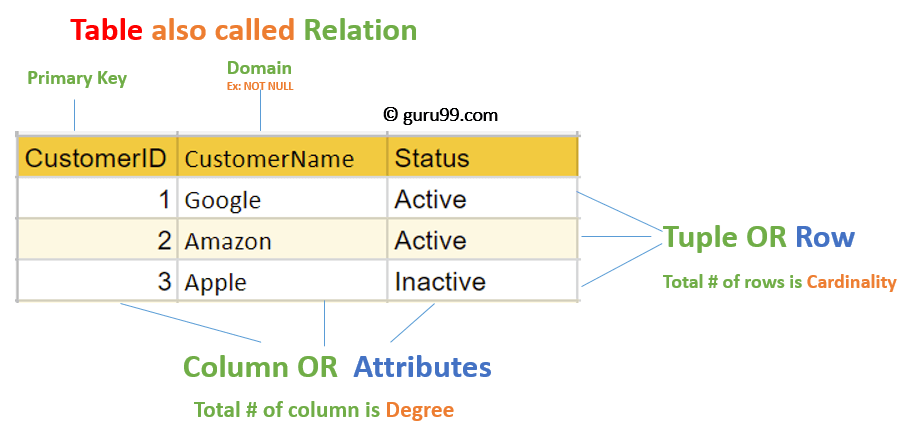
\includegraphics[width=\linewidth]{RelationalModel.jpg}
    \caption{Relational Model}
\end{figure}

\begin{description}
    \item[Attribute] Column
    \item[Relation] Table
    \item[Tuple] Row
    \item[Degree] Count(Column)
    \item[Cardinality] Count(Row)
    \item[Domain] 数据类型,约束等
    \item[Relation Key] 主键外键
    \item[Relation Schema] 表名 和 其中的列
    \item[Relation Instance] 表中的数据
\end{description}


\subsection{SQL}

Data Definition Language 定义

\begin{itemize}
    \item CREATE
    \item ALTER
    \item DROP
    \item TRUNCATE
\end{itemize}

Data Manipulation Language 操作

\begin{itemize}
    \item INSERT
    \item UPDATE
    \item DELETE
\end{itemize}

Data Control Language 权限

\begin{itemize}
    \item GRANT
    \item REVOKE
\end{itemize}

Transaction Control Language 事务

\begin{itemize}
    \item COMMIT
    \item ROLLBACK
    \item SAVEPOINT
\end{itemize}

Data Query Language 查询

\begin{itemize}
    \item SELECT
\end{itemize}


\subsection{索引}

Clustered Index

\begin{itemize}
    \item 行的物理与逻辑顺序相同
    \item 一个表只有一个
    \item Primary Key 默认
\end{itemize}

Nonclustered Index

\begin{itemize}
    \item 储存的是指向行的指针
    \item UNIQUE 默认
\end{itemize}

Covering Indexes

\begin{itemize}
    \item 索引中包含了要查询的字段
\end{itemize}


\subsection{Normalization}

消除冗余,inconsistent 的依赖关系


\subsubsection{不一致}

用户在 Customer 表中查找 Address 是合理的  
但是在这里查找 负责这个客户的 员工的 Salary 就不合理了  
这应该去 Employee 表中查找

不一致的依赖关系 会使数据难以访问

\begin{table}[H]
    \centering
    \begin{tabular}{|c|c|c|c|c|c|}
        \hline
        学号 & 教师 & 咨询室 & 课程 1 & 课程 2 & 课程 3 \\
        \hline
        S1 & T1 & R1 & C1 & C2 & C3 \\
        \hline
        S2 & T2 & R2 & C1 & C2 & C4 \\
        \hline
    \end{tabular}
\end{table}


\subsubsection{1NF}

每一个字段都是最小的,不包含其他字段,不重复

\begin{itemize}
    \item 消除重复的列
    \item 为相关数据单独建表
    \item 使用主键标识每组相关数据
\end{itemize}

\begin{table}[H]
    \centering
    \begin{tabular}{|c|c|c|c|}
        \hline
        学号 & 教师 & 咨询室 & 课程 \\
        \hline
        S1 & T1 & R1 & C1 \\
        \hline
        S1 & T1 & R1 & C2 \\
        \hline
        S1 & T1 & R1 & C3 \\
        \hline
        S2 & T2 & R2 & C1 \\
        \hline
        S2 & T2 & R2 & C2 \\
        \hline
        S2 & T2 & R2 & C4 \\
        \hline
    \end{tabular}
\end{table}


\subsubsection{2NF}

消除重复的行

\begin{itemize}
    \item 为应用于多条记录的值,创建单独的表
    \item 用外键连接这些表
\end{itemize}

Student

\begin{table}[H]
    \centering
    \begin{tabular}{|c|c|c|}
        \hline
        学号 & 教师 & 咨询室 \\
        \hline
        S1 & T1 & R1 \\
        \hline
        S2 & T2 & R2 \\
        \hline
    \end{tabular}
\end{table}

Course

\begin{table}[H]
    \centering
    \begin{tabular}{|c|c|}
        \hline
        学号 & 课程 \\
        \hline
        S1 & C1 \\
        \hline
        S1 & C2 \\
        \hline
        S1 & C3 \\
        \hline
        S2 & C1 \\
        \hline
        S2 & C2 \\
        \hline
        S2 & C4 \\
        \hline
    \end{tabular}
\end{table}


\subsubsection{3NF}

消除与主键无关的数据:咨询室是与学生编号无关的数据

Student

\begin{table}[H]
    \centering
    \begin{tabular}{|c|c|}
        \hline
        学号 & 教师 \\
        \hline
        S1 & T1 \\
        S2 & T2 \\
        \hline
    \end{tabular}
\end{table}

Teacher

\begin{table}[H]
    \centering
    \begin{tabular}{|c|c|}
        \hline
        教师 & 咨询室 \\
        \hline
        T1 & R1 \\
        T2 & R2 \\
        \hline
    \end{tabular}
\end{table}


\subsubsection{Boyce-Codd}

在 3NF 的基础上,每个属性都不传递依赖

StorehouseManage (WarehouseID, ItemID, AdminID, Num)

每个管理员只在一个仓库工作,一个仓库储存多个物品,则存在关系

\begin{itemize}
    \item (WarehouseID, ItemID) $\to$ (AdminID, Num)

    \item (AdminID, ItemID) $\to$ (WarehouseID, Num)
\end{itemize}

所以有两组候选关键字,唯一非关键字是 Num,符合 3NF,但是存在 (WarehouseID) $\leftrightarrow$ (AdminID) 关键字决定关键字的情况,循环传递依赖

异常:

\begin{description}
    \item[删除] 清空仓库会导致 WarehouseID AdminID 被删除

    \item[插入] 仓库无物品时,无法分配管理员

    \item[更新] 换管理员,则修改全表
\end{description}

修改:

\begin{itemize}
    \item StoreManage (WarehouseID, AdminID)

    \item Warehouse (WarehouseID, ItemID, Num)
\end{itemize}


\subsubsection{4NF}

消除 Multi-Valued Dependency,最简单的是多对多


\subsection{Entity Relationship}

\begin{description}
    \item[Entity] 矩形,表
    \item[Attribute] 椭圆,列
    \item[Relationship] 菱形,表之间的关系
    \item[Computed] 虚线,计算得出的属性
    \item[Multi Value] 双椭圆,多值属性
    \item[Optional] 可选属性
    \item[Composite] 矩形内加一个菱形,多对多联系
    \item[Weak] 双层矩形,依赖另一个实体存在
\end{description}

\begin{figure}[H]
    \centering
    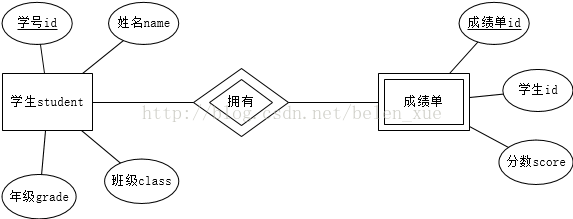
\includegraphics[width=\linewidth]{ER2.png}
\end{figure}

\begin{figure}[H]
    \centering
    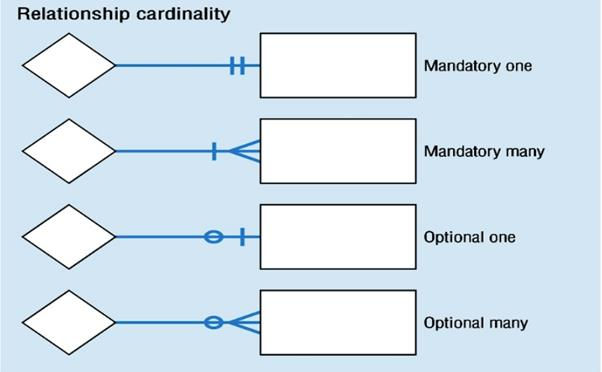
\includegraphics[width=\linewidth]{ER.jpg}
\end{figure}

画图步骤

\begin{enumerate}
    \item Entity Identification 找实体
    \item Relationship Identification 找关系
    \item Cardinality Identification 一对多之类的
    \item Identify Attributes 找列
    \item Create ER Diagram 画图
\end{enumerate}


\subsection{数据仓库}

Online Analytical Processing,使用数据库系统来帮助洞察业务,如 Redshift,主要用于数据分析

数据仓库是为只读优化的

\begin{description}
    \item[事实表] 含有大量的数据,并且是可以汇总,并被记录的

    \item[维度表] 分析数据的窗口,包含事实表中记录的属性

    \item[Star] 一张事实表和多张维度表组成

    \item[Snowflake] 每一个维度表都可以向外连接多个子维度表

    \item[Galaxy] 多个事实表版本的星型模型,多张事实表共用模型中的维度表
\end{description}


\subsubsection{Data Cube}

表示那些很大的数据集合,储存多维度数据

\begin{figure}[H]
    \centering
    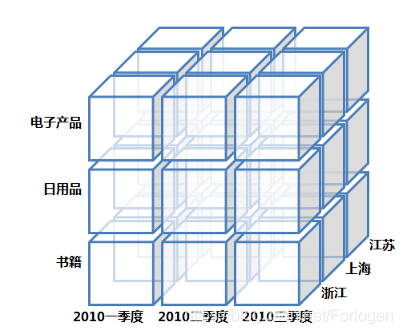
\includegraphics[width=\linewidth]{Cube.png}
\end{figure}

\begin{description}
    \item[Drill Down] 季度总销售 $\to$ 每个月

    \item[Roll Up] 4 5 6 月 $\to$ 第二季度

    \item[Slice] 只分析电子产品

    \item[Dice] 第一和第二季度

    \item[Rotate] 产品与地区互换维度
\end{description}

\begin{figure}[H]
    \centering
    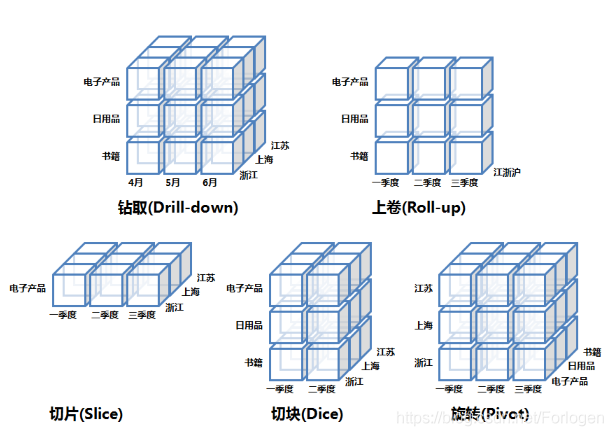
\includegraphics[width=\linewidth]{Action.png}
\end{figure}


\section{Algorithms \& Data Structures}


\section{Graph Algorithms}


\section{Programming}


\section{Compilers}


\section{System Engineering}


Mathematics


\section{Set}


\section{Logics}


\section{Linear Algebra}


\section{Calculus}


\section{Probability}


\section{Numerical}


\end{document}
